%!TEX root = ../../tfg.tex
\chapter{Libro de arte}

\section{Consideraciones sobre el material artístico}

El contenido presentado en este apéndice se incluye únicamente como material
complementario de la memoria. Su finalidad es mostrar parte del trabajo visual que
acompaña al videojuego y facilitar una visión más completa de su identidad gráfica.

La elaboración de estos recursos artísticos no forma parte del alcance evaluado del TFG.
Por tanto, el tiempo dedicado a dibujar, revisar o adaptar estos sprites no se contabiliza
dentro de la planificación, seguimiento ni estimación de esfuerzo del proyecto.

\section{Logotipo}

\begin{figure}[H]
    \centering
    
\includegraphics[width=.55\textwidth]{figures/sprites/logo_red.png}
    \caption{Logotipo de \textit{Via Inferni}.}
    \label{fig:sprites-logo}
\end{figure}

\section{Personajes y armas}

\begin{figure}[H]
    \centering
    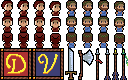
\includegraphics[width=.7\textwidth]{figures/sprites/characters_and_weapons.png}
    \caption{Sprites de personajes principales y armas.}
    \label{fig:sprites-characters-weapons}
\end{figure}

\section{Objetos y elementos interactivos}

\begin{figure}[H]
    \centering
    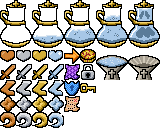
\includegraphics[width=.75\textwidth]{figures/sprites/items_and_others.png}
    \caption{Sprites de objetos, recompensas y otros elementos interactivos.}
    \label{fig:sprites-items}
\end{figure}

\section{Enemigos}

\begin{figure}[H]
    \centering
    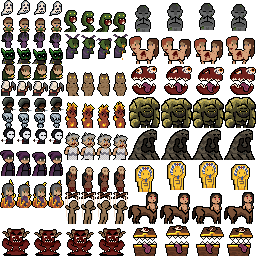
\includegraphics[width=.85\textwidth]{figures/sprites/all_enemies.png}
    \caption{Conjunto de sprites de enemigos diseñados para el juego.}
    \label{fig:sprites-enemies}
\end{figure}

\section{Tileset}

\begin{figure}[H]
    \centering
    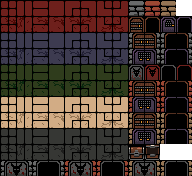
\includegraphics[width=.85\textwidth]{figures/sprites/tileset.png}
    \caption{Tileset utilizado para la construcción visual de las salas.}
    \label{fig:sprites-tileset}
\end{figure}
